
\setcounter{chapter}{-1}
\chapter{Appendices} \label{appendix}
\renewcommand{\thechapter}{A}

%%%%%%%%%%%%%%%%%%%%%%%%%%%%%%%%%%%%%%%%%%%%%%%%%%%%
%%%%%%%%%%%%%%%%%%%%%%%%%%%%%%%%%%%%%%%%%%%%%%%%%%%%

\section{Additional publications} \label{app:paper}
The following pages present the manuscript:
Kepiro, I. E., Marzuoli, I., Hammond, K., et al. Engineering chirally blind protein pseudo-capsids into nanoprecise antibacterial persisters, submitted to ACS Nano and currently under revision. Chapter \ref{chapter:capzip_results} includes part of the results presented in the paper, elaborating them further.

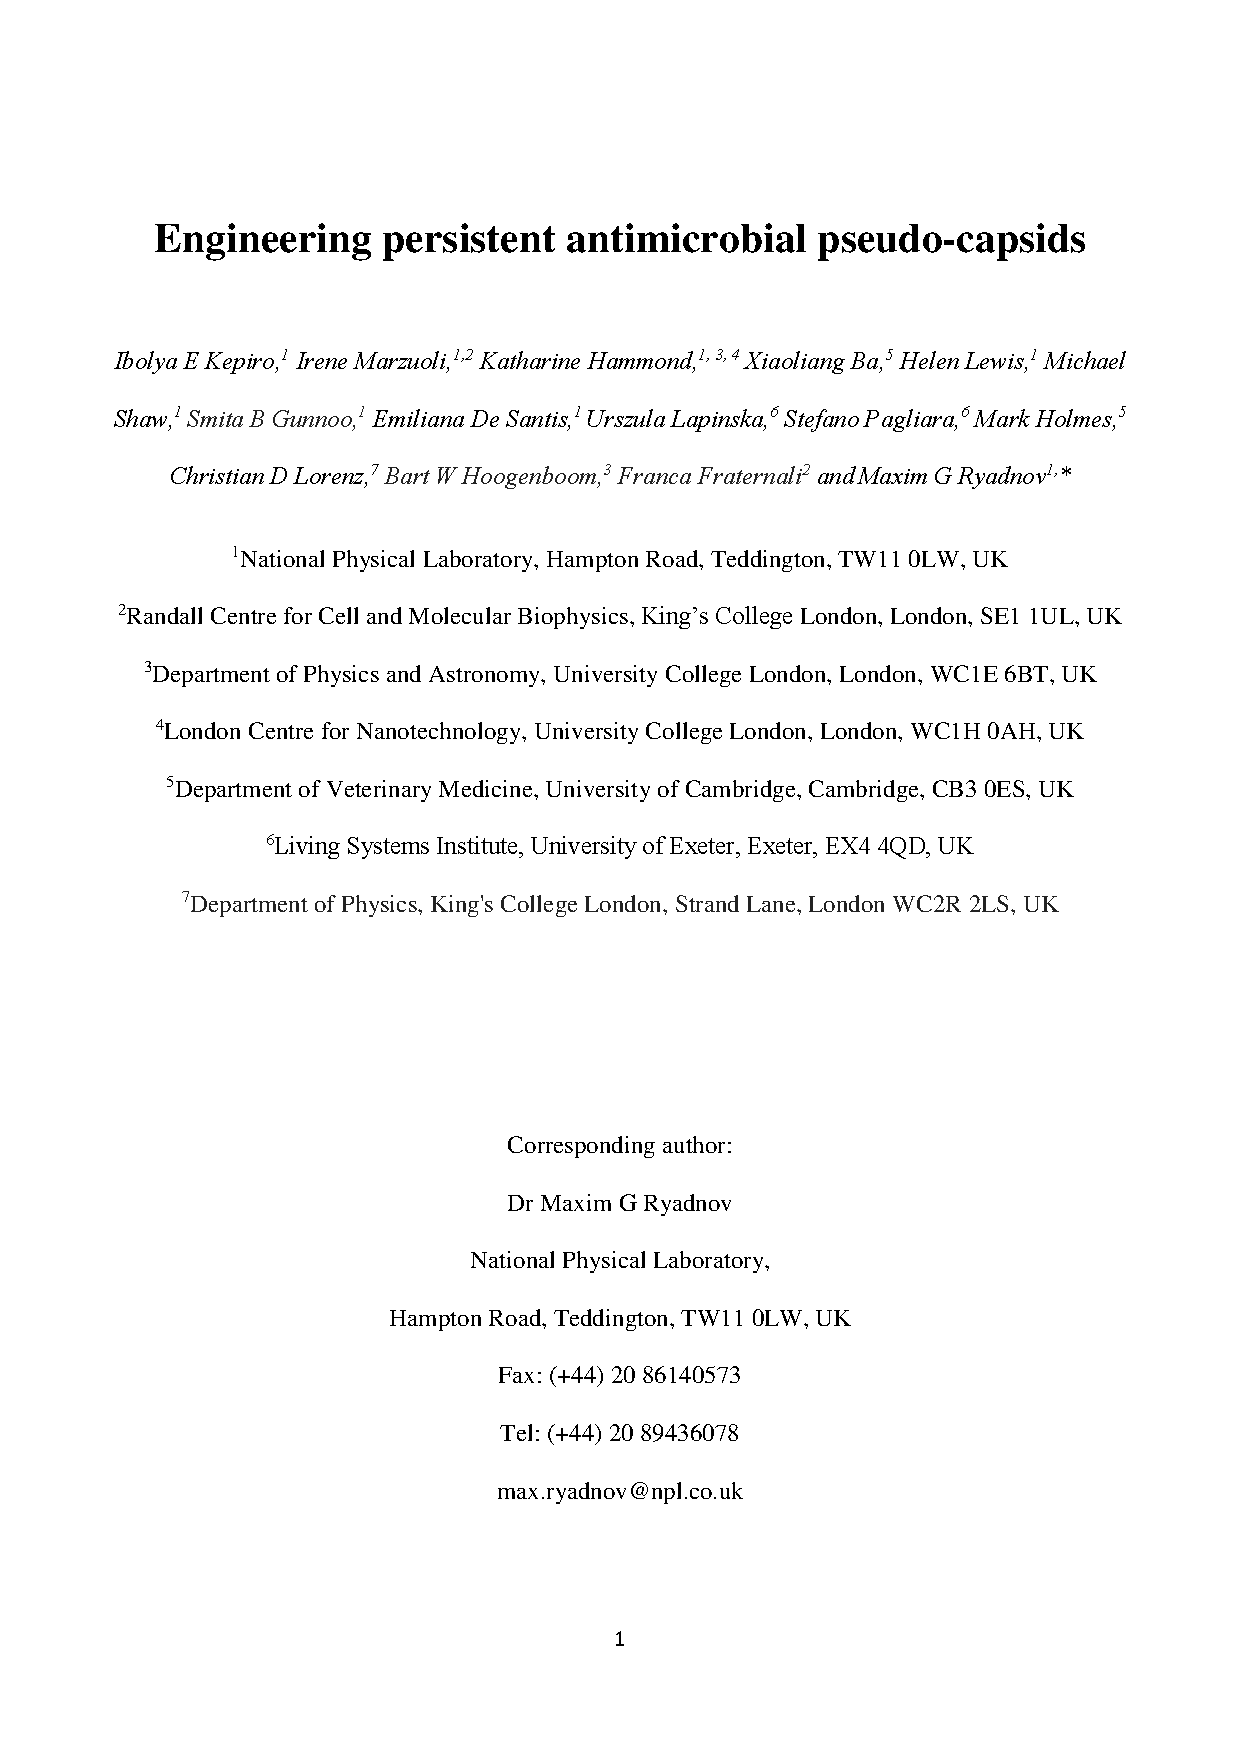
\includepdf[pages=1-25, nup=1x2, offset = 5mm 0mm, scale = 0.8, pagecommand = \pagestyle{thesis}, landscape = true]{Kepiro_et_al.pdf}
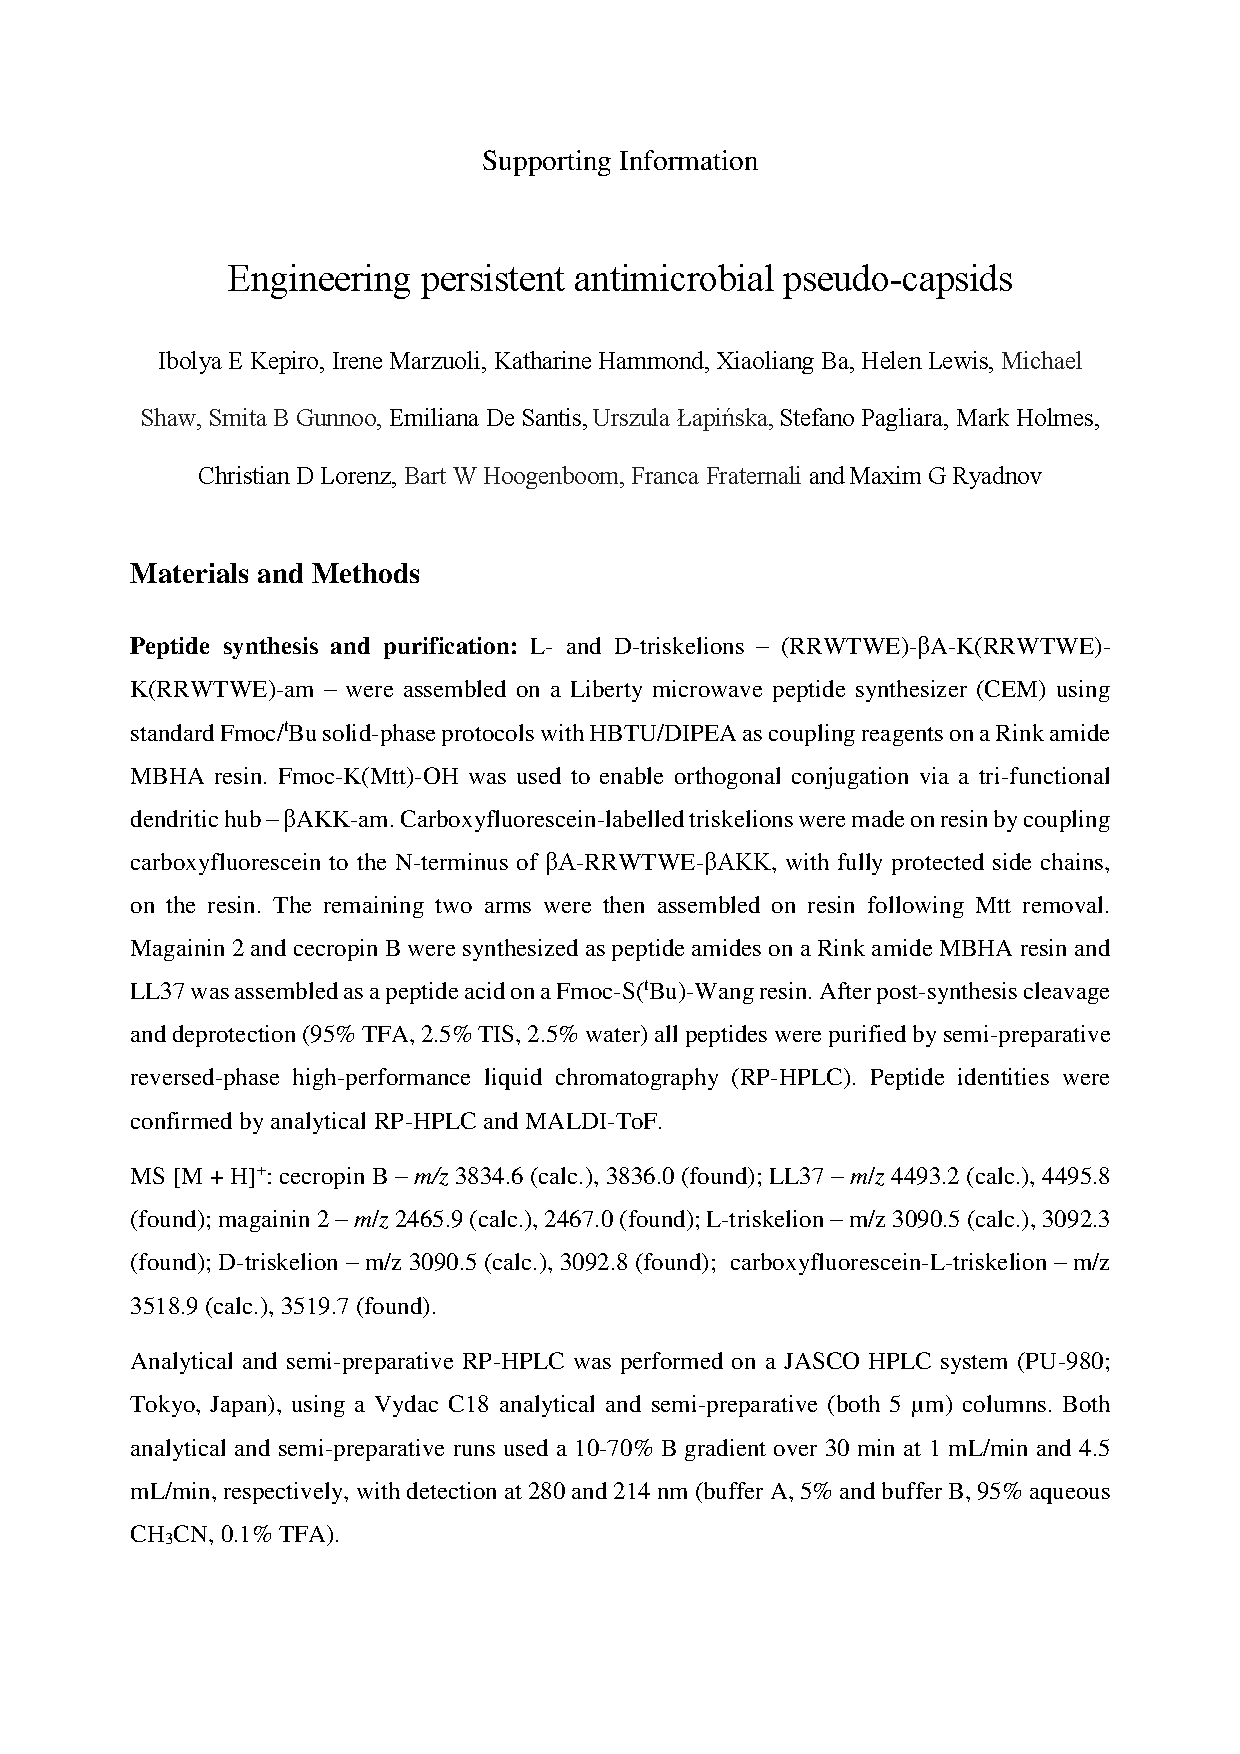
\includepdf[pages=1-13, nup=1x2, offset = 5mm 0mm, scale = 0.8, pagecommand = \pagestyle{thesis}, landscape = true]{Kepiro_et_al_SI.pdf}


\section{Supplementary material}
\label{sec:SI}
Supplementary material can be found at \url{https://github.com/imarzuoli/????} and includes Supplementary Movies of:
\begin{itemize}
\item \url{SI_M1_GROMOS_buckyball.mp4} \\ GROMOS atomistic simulation of the buckyball bilayer - 100 ns;

\item \url{SI_M2_SIRAH_buckyball.mpg} and \url{SI_M3_PolarMARTINI_buckyball.mpg} \\ SIRAH and Polar MARTINI coarse-grained simulations of the buckyball bilayer and monolayer - 1 $\mu$s;

\item \url{SI_M4_GROMOS_capzip_bacterial_E130_poration.mp4} \\ atomistic simulation of poration of a model bacterial model membrane under the combined action of the pentagonal capzip subunit and an external electric field of 130 mV/nm - 60 ns;

\item \url{SI_M5_MARTINI_capzip_bacterial.mp4} and \url{SI_M6_MARTINI_capzip_mammalian.mpg} \\ standard MARTINI simulation of a buckyball bilayer approaching a bacterial and mammalian model membrane - 10 $\mu$s;

\item \url{SI_M7_PolarMARTINI_capzip_bacterial_E40_poration.mpg} \\ Polar MARTINI simulation of a buckyball bilayer porating a model bacterial membrane under the effect of a 40 mV/nm external electric field - 200 ns.
\end{itemize}


\clearpage
\section{Software developed}
\label{sec:Appendix_software}

The simulations and analysis of capzip systems prompted the development of tools to facilitate the task.
%
These are meant to be used in conjunction with standard analysis tools provided by GROMACS \citep{Berendsen1995,Abraham2015,gromacs_man} and MDAnalysis \citep{Michaud-Agrawal2011,Gowers2016}.
%
The scripts and packages developed can be found at \url{https://github.com/imarzuoli/MDtools}, which includes:
\begin{itemize}
\item python functions to perform the analysis of contacts as in Section \ref{sec:results_cap} of Chapter \ref{chapter:capzip_results} (\url{contacts_analysis.py});

\item functions to perform the hydration analysis as in Section 3.4 of Chapter \ref{chapter:lip_par} (\url{an_min_hist.py});
%\emph{delete_water.py}: a script to delete water molecules in a given slice of space (perpendicular to either x, y or z)

\item a python module to manipulate multi-branched peptide topology files in the GROMACS format for GROMOS simulations (\url{MD_mutate_and_manipulate.py}).

\end{itemize}
